\chapter{Progettazione e implementazione}
% [titolo ridotto se non ci dovesse stare] {titolo completo}
%

\begin{citazione}
    In questo capitolo vengono illustrate tutte le componenti principali di un motore scacchistico e vengono discussi gli approcci alla realizzazione delle stesse.
\end{citazione}

\newpage
\section{Rappresentazione della scacchiera e dei pezzi}

\subsection{Introduzione} %\label{1sec:scopo}
Il primo passo dello sviluppo di un motore scacchistico è decidere come si vuole rappresentare
la scacchiera , si tratta di una scelta fondamentale, non solo perché in seguito ci permetterà
di testare le funzioni che andremo a implementare, ma anche perché è nella scacchiera che , generalmente,
viene conservato lo stato generale della partita.\footnote{per stato di una partita si intendono informazioni come
    informazioni su chi ha diritto di muovere, i permessi di arrocco,lo stato della regola delle 50 mosse etc}
\\Inoltre il tipo di codifica può influenzare la rapidità
e la facilità col quale possiamo accedere alle informazioni sullo stato corrente dei pezzi
e come vedremo in seguito è in grado di influenzare funzioni come la generazione delle mosse, per questi motivi,
non è raro per motori scacchistici particolarmente complessi l'utilizzo di più tipi di strutture dati in base
al tipo di informazione da conservare e all'utilizzo che se ne vuole fare, spesso alternando tra strutture efficienti dal punto di vista computazionale (bitboard) a strutture che permettono l'accesso casuale o facilitano 
operazioni di manipolazione da parte di un programmatore umano (qualsiasi rappresentazione casellocentrica).
\\Per la rappresentazione di una scacchiera sono chiaramente possibili moltissime scelte, di seguito
verranno illustrate alcune tra le più famose ed utilizzate.

\subsection{Rappresentazione della scacchiera Pezzocentrica}
Si definisce rappresentazione pezzocentrica, un qualsiasi tipo di rappresentazione della scacchiera che mantiene liste
array o set dei pezzi attualmente presenti sulla scacchiera con annesse le informazioni sulle caselle da essi occupate.
Le rappresentazioni più comuni sono:
\subsubsection{Piece-Lists}
liste o array di ogni pezzo sulla scacchiera, ogni elemento della lista o dell'array associa un pezzo
alla casella che esso occupa .Le caratteristiche di ogni pezzo (colore,tipo etc)
possono essere associate all'indice dell'array in cui si trovano o essere presenti in ulteriori array
o liste esterne.

\subsubsection{Bitboards}
Una Bitboard è una struttura dati specifica per i giochi da tavolo,
si tratta in sostanza  di una struttura dati in grado di immagazzinare lo stato di ogni casella della
scacchiera all'interno di una parola\footnote{Una parola è un gruppo di bit di una determinata dimensione che sono gestiti come unità dal set di istruzioni o dall'hardware di un processore} di 64 bit\cite{Bitboard}.
\\Vediamo un esempio pratico, immaginiamo di avere una scacchiera che si trova nello stato di default di inizio
partita come nella figura \ref{scacchiera}, una bitboard tipica è quella che ci permette di sapere in quali caselle è presente un pedone
nero,per costruirla, operando casella per casella, ci poniamo una domanda "in questa casella
è presente un pedone nero?" se si allora quella casella viene marcata con un 1 , altrimenti viene
marcata con uno 0, la bitboard che codifica questa informazione sarà quindi la parola di 64 bit 00000000 11111111 00000000 00000000 00000000
00000000 00000000 00000000 come si può vedere in \ref{scacchiera}.:
\begin{figure}
    \centering
    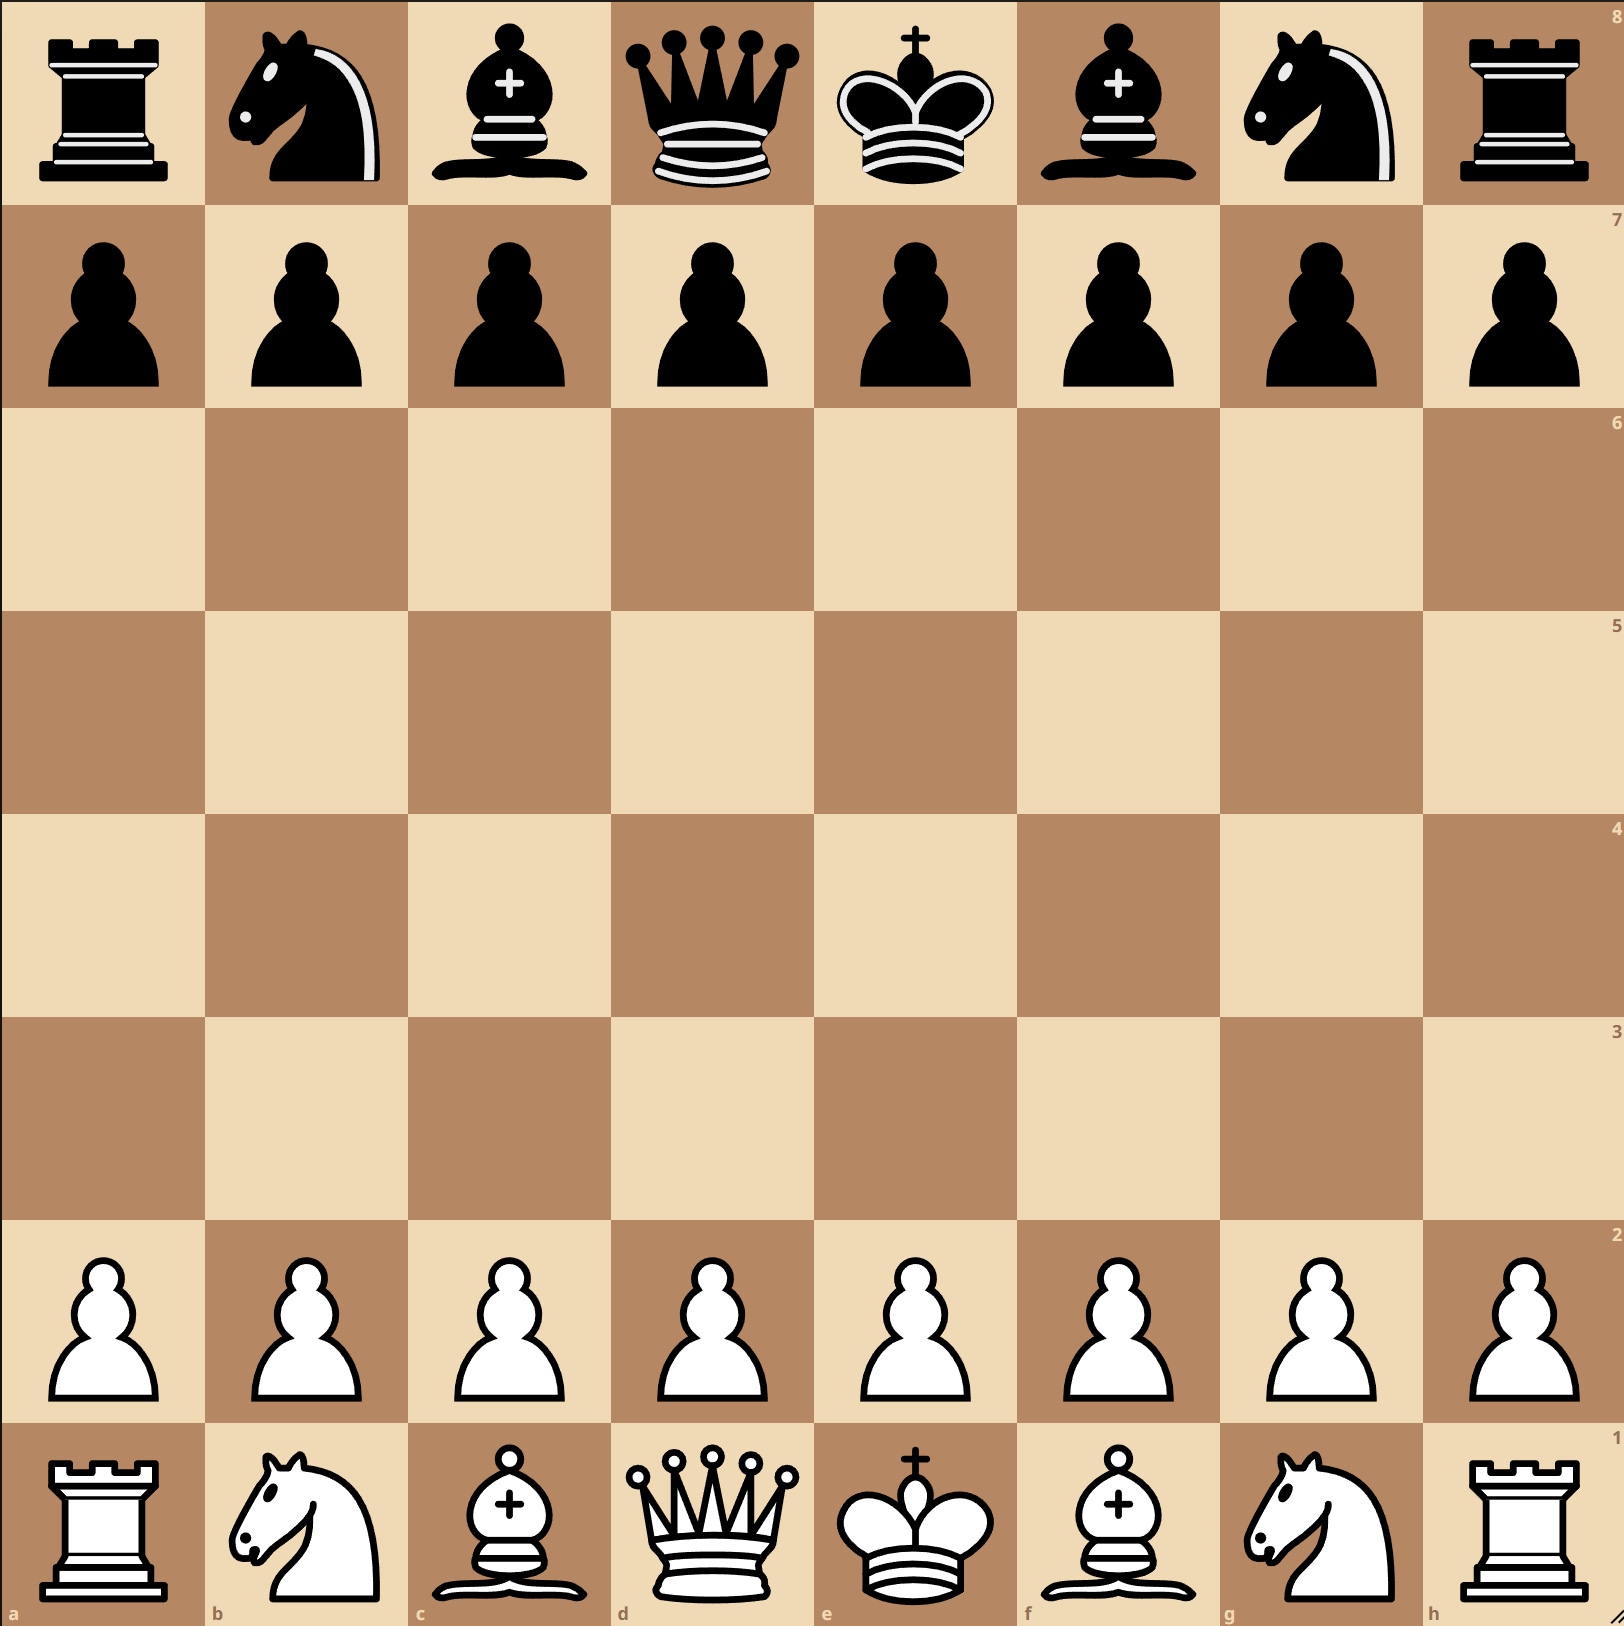
\includegraphics[width=\linewidth/2] {scacchiera.png}
    \caption{Scacchiera nella posizione iniziale di gioco }
\end{figure}


\begin{figure}[h!]
    \centering
    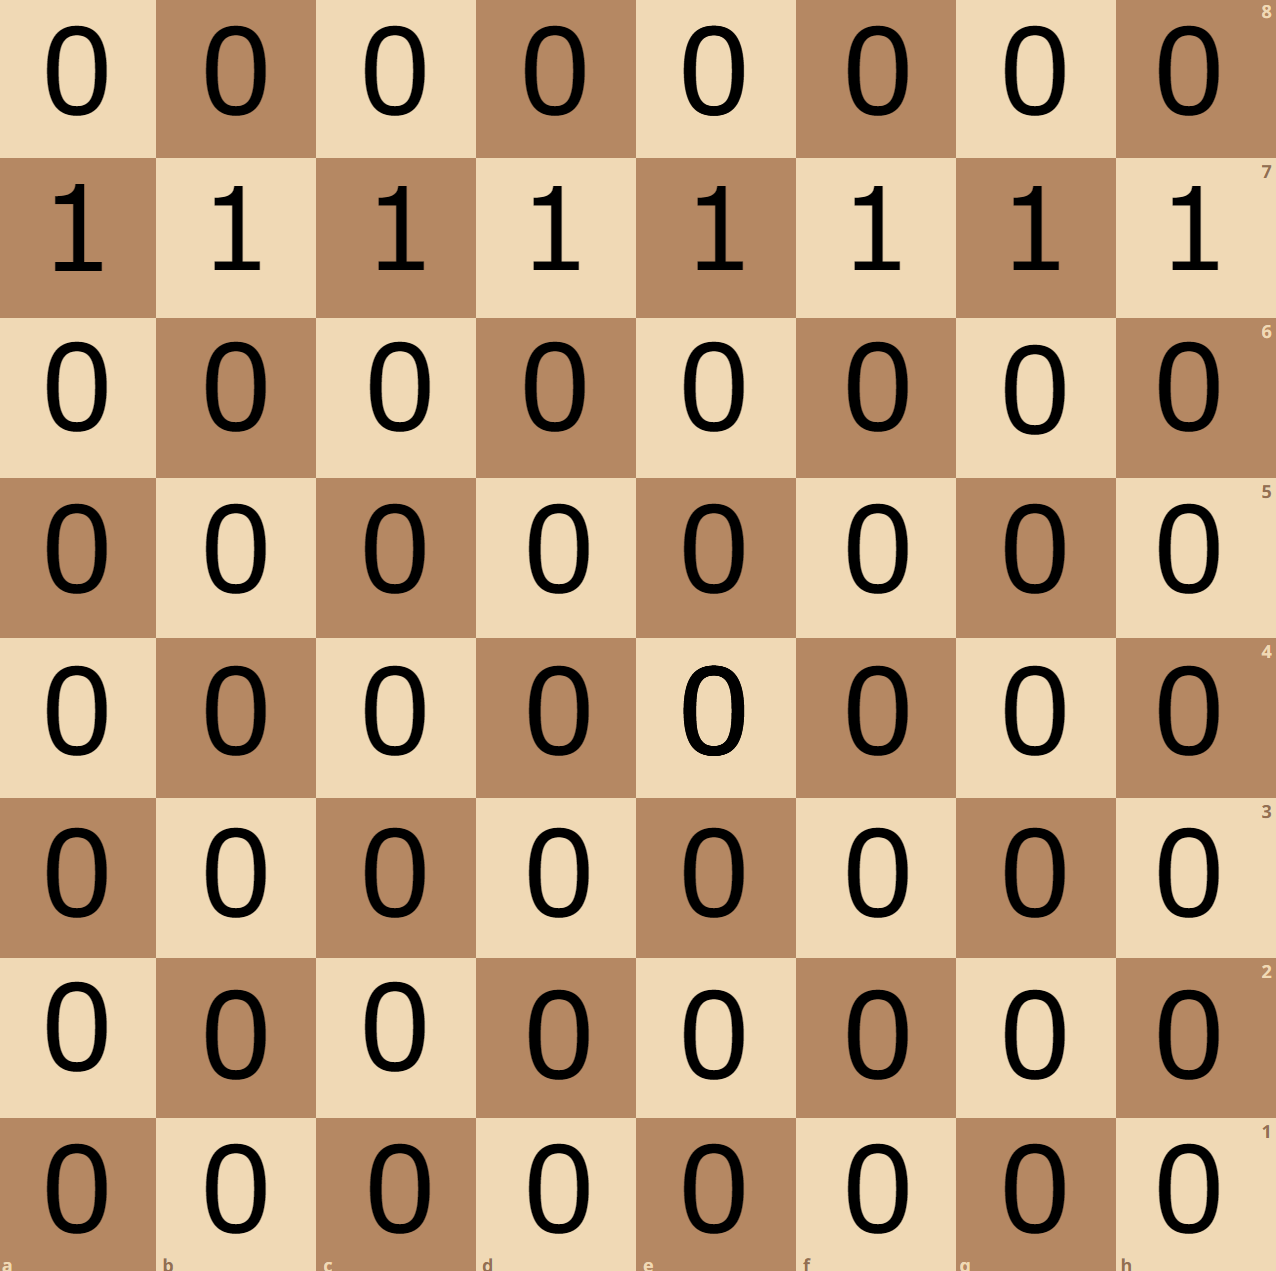
\includegraphics[width=\linewidth/11*5] {bitboard.png}
    \caption{bitboard}
    \label{scacchiera}
\end{figure}


\subsubsection{Piece-Sets}
Rappresentazione con set con un bit per ogni pezzo dentro una parola a 32 bit o 2 parole a 16 bit per ogni lato,
i Piece-sets hanno  delle somiglianze con le bitboards, ma ogni  bit del set non è   direttamente correlato ad una casella,
ma ad un indice  dentro ad una  piece-list. Spesso la posizione del bit nella parola di un  piece-set  implica
, di che tipo e colore il pezzo è, mentre le  bitboards solitamente mantengono set distinti per pezzi diversi.




\subsection{Rappresentazione della scacchiera Casellocentrica}
La rappresentazione casellocentrica  mantiene un associazione inversa rispetto a quella pezzocentrica,
per ogni casella conserviamo in memoria se è vuota o occupata da un pezzo in particolare.
La macro-categoria di  rappresentazione più comune è la Mailbox:

\subsubsection{Mailbox}
La rappresentazione Mailbox è una rappresentazione casellocentrica dove la codifica di ogni casella risiede in una struttura dati
che permette l'accesso casuale, solitamente si utilizza un array con l'indice che codifica dal numero della casella in array monodimensionali
o dalla coppia traversa/colonna\footnote{termini scacchistici per indicare le righe e le colonne della scacchiera} in array bidimensionali.
Il nome deriva dall'associazione di ogni indice al concetto di "indirizzo" di una casella postale.Le implementazioni più famose e
comuni del concetto di Mailbox sono la 8x8 Board e la 10x12 Board.

\subsubsection{8x8 Board}
Una board 8x8, è una rappresentazione pezzocentrica consistente  in un array mono o bidimensionale di bytes o interi, contenenti rappresentazioni codificate
per i pezzi e per la casella vuota, con i due indici ricavati o dalla coppia traversa/colonna che identifica la casella sulla scacchiera ,
o più comunemente  da 0 a 63, uno per ogni casella della scacchiera.
Questo tipo di rappresentazione è usata spesso come rappresentazione ridondante all'interno di programmi che utilizzano bitboards
per individuare se e quali pezzi sono presenti su una casella in maniera efficiente.

\subsubsection{10x12 Board}
Una board 10x12 visibile nella figura \ref{10x12} contorna una board 8x8 con traverse e colonne sentinelle per individuare indici al di fuori della scacchiera durante la generazione delle mosse, anche questo tipo di board 
come la 8x8 di cui è un derivativo, può essere usata per accedere in maniera efficiente e facile per un programmatore umano a specifiche caselle della scacchiera per individuare o meno la presenza di pezzi.
\vfill
\begin{figure}[!ht]
    \centering
    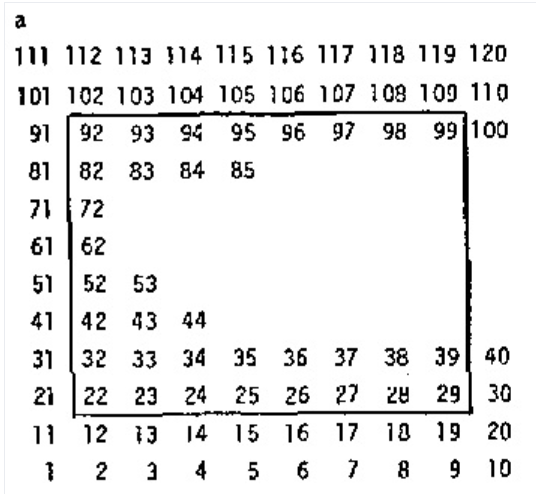
\includegraphics[width=\linewidth/2]{10x12 board.png}
    \caption{Rappresentazione di una board 10x12,notare come le 2 traverse extra sopra e sotto siano necessarie per evitare accessi out of bounds in caso di cavalli posizionati sulla prima o ottava fila }
    \label{10x12}
\end{figure}



\subsubsection{Rappresentazione dei pezzi}
Una volta scelto il tipo di rappresentazione della scacchiera si può iniziare a pensare alla rappresentazione dei pezzi,
anche se può sembrare controintuitivo i pezzi non hanno bisogno di una struttura elaborata, la generazione delle possibili
mosse verrà gestita nella move generation ed il loro spostamento all'interno della scacchiera verrà gestito da una funzione monolitica, in grado di distinguere autonomamente i pezzi, solitamente chiamata
MakeMove, per i pezzi quindi abbiamo bisogno di una
rappresentazione semplice, di facile interpretazione e che occupi poco spazio.\\Rappresentazioni molto comuni sono quella
tramite interi, dove ad ogni tipo di pezzo viene assegnato un numero che funge da identificativo univoco e quella tramite
caratteri, dove ad ogni tipo di pezzo viene assegnato un carattere che lo identifica (e che in linguaggi come il C è funzionalmente identica a quella per interi).


\section{Move Generation}
\label{move generation} %\label{1cap:spinta_laterale}
% [titolo ridotto se non ci dovesse stare] {titolo completo}
%
Una volta stabilito il tipo di rappresentazione il passo successivo è quello della generazione delle mosse, per generazione delle mosse si intende la generazione
di tutte le mosse legali eseguibili data una posizione di partenza, la generazione delle mosse è un processo fondamentale in quanto identifica i rami che
il nostro algoritmo potrà esplorare nella successiva fase, quella appunto di ricerca, trattata nel paragrafo \ref{ricerca}.



\subsection{Approcci alla generazione delle mosse}
La generazione delle mosse viene affrontata con 3 approcci radicalmente diversi a seconda del tipo di pezzo che stiamo trattando, in particolare la distinzione si effettua tra 
pedoni,pezzi scorrevoli (alfieri,torri,regine) e non scorrevoli(re e cavalli).

\subsubsection{Pedoni}
Il pedone muove solo in avanti, mai indietro o di lato e può avanzare  di due caselle se è la prima volta che viene mosso,altrimenti può avanzare solo di una.
\\Il un pedone mangia un pezzo avversario spostandosi diagonalmente di una casella,sempre soltanto in avanti, o a destra o a sinistra, se un pedone raggiunge la traversa finale della scacchiera rispetto alla sua direzione di movimento
allora viene promosso, diventa quindi,a scelta del giocatore che possiede la pedina, uno qualsiasi degli altri pezzi  (ad eccezione del re).
In un approccio basato su board 8x8 o 12x10 possiamo calcolare le possibili mosse del pedone affidandoci a un flag che rappresentano la possibilità di effettuare catture en passant e controllare la possibilità 
di muovere di 2 caselle e di promozione basandoci sulla posizione di partenza del pedone,le caselle di arrivo possibili sono a quel punto calcolabili sommando alla casella di partenza degli offset prefissati.



\subsubsection{Pezzi non scorrevoli}
I pezzi non scorrevoli sono i pezzi che possono spostarsi solo di un numero finito e fisso di caselle,questo vuol dire che,conoscendo il tipo e la posizione di un pezzo non scorrevole,possiamo calcolare i suoi movimenti
sommando alla sua posizione dei valori prefissati,a quel punto dovremo solo assicurarci che la casella di arrivo sia nei limiti della scacchiera e che la mossa risultante sia legale\footnote{Nel gioco degli scacchi una mossa illegale è una mossa che pone il re sotto scacco o non libera il re da uno scacco subito alla mossa precedente}.

\subsubsection{Pezzi  scorrevoli}
Si definiscono pezzi scorrevoli i pezzi che possono spostarsi di un numero non prefissato di caselle lungo l'asse orizzontale,verticale o diagonale,fino a raggiungere il bordo della scacchiera o un altro pezzo
e nel gioco degli scacchi consistono di alfiere,torre e regina.La generazione delle mosse di questo tipo di pezzi è più complessa rispetto a quella degli altri pezzi, in quanto bisogna controllare la presenza di pezzi,propri
o avversari che siano, in grado di fermare il movimento del pezzo e bisogna assicurarsi che il pezzo non superi il bordo della scacchiera;
nel corso  dei decenni si è arrivati a stabilire due approcci alla progettazione ottimali per la generazione delle mosse dei pezzi scorrevoli, 
da preferire in base all'architettura della macchina che esegue il motore.

\subsubsection{Bitboard magiche}
L'approccio con le bitboard magiche consiste nell'assegnare ad ogni pezzo scorrevole un numero "magico" pre-calcolato per ogni casella della scacchiera, rappresentata da una bitboard, quel numero verrà poi moltiplicato
 per il valore individuato dalla posizione dei pezzi bloccanti sulla scacchiera, ottenuto settando ad 1 ogni pezzo che per primo blocca il movimento di un pezzo in una data direzione di spostamento , come 
 visibile nelle  figure \ref{aaa} e \ref{bbb}.\\  
Questa moltiplicazione darà luogo ad un indice con il quale accedere ad un archivio di bitboard di 
attacco\footnote{bitboard che segnala con dei bit ad 1 quali caselle il pezzo può attaccare} pre-calcolate, si tratta di una soluzione meno efficiente rispetto alle bitboard che si basano sull'utilizzo di pext
e va utilizzata solo in caso di architetture che non supportano nativamente il set di istruzioni BMI2.


\begin{figure}
    \centering
    \begin{minipage}{0.45\textwidth}
        \centering
        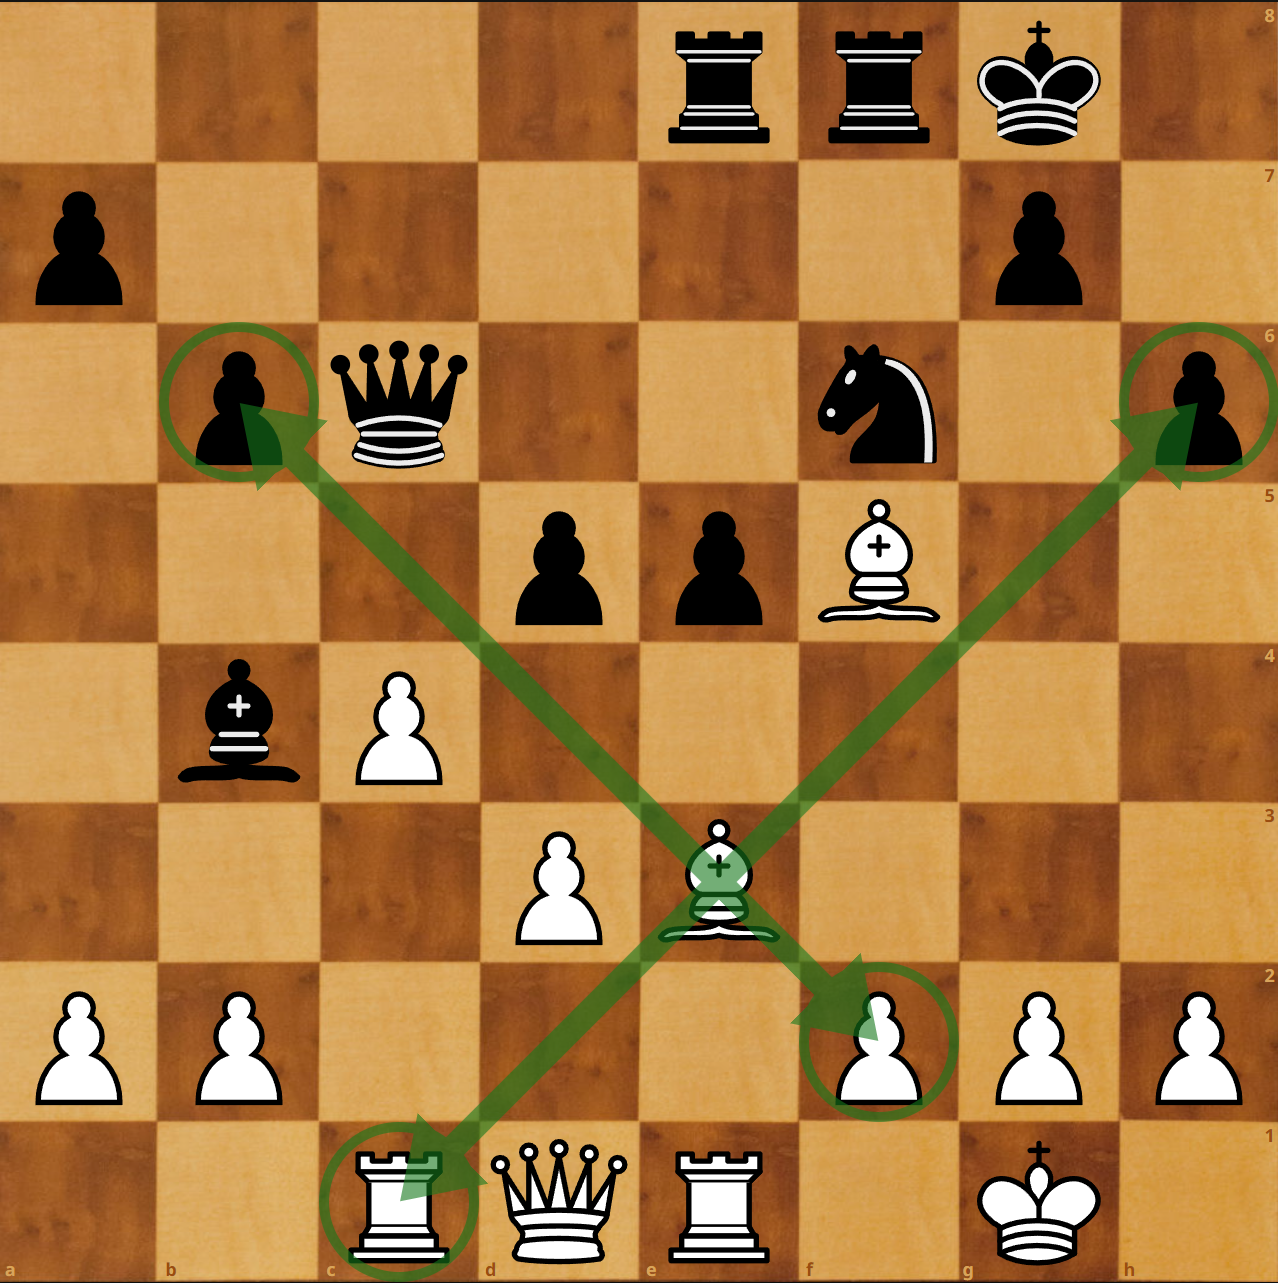
\includegraphics[width=0.9\textwidth]{alfiere.png} % first figure itself
        \caption{posizione d'esempio su una scacchiera}
        \label{aaa}
    \end{minipage}\hfill
    \begin{minipage}{0.45\textwidth}
        \centering
        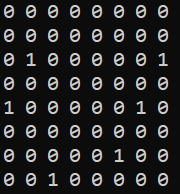
\includegraphics[width=0.8\textwidth]{occupancy.png} % second figure itself
        \caption{Bitboard di occupazione che codifica la figura 2.4}
        \label{bbb}
    \end{minipage}
\end{figure}




\subsubsection{PEXT Bitboards}
Una bitboard pext funziona in maniera simile ad una bitboard magica,utilizza il valore individuato dalla posizione dei pezzi bloccanti sulla scacchiera sulla bitboard per generare un indice da usare per accedere ad una
bitboard di attacco,la differenza sostanziale però è nell'approccio, una bitboard pext, come intuibile dal nome, utilizza l' istruzione pext introdotta nel set di istruzioni BMI2 da intel sui processori haswell,e con 
la serie 5000 dei processori ryzen da AMD,si tratta di un'istruzione che ,dato un input ed una maschera,trasferisce i bit dell'input individuati dalla maschera,in ordine contiguo e da destra a sinistra.
Con l'istruzione pext, usando una bitboard che rappresenta la scacchiera come input e la posizione dei pezzi bloccanti come maschera, si può ottenere un indice per la hash table delle bitboard di attacco,il tutto viene eseguito in un solo ciclo 
di cpu e risulta quindi molto più efficiente di un approccio con bitboard magiche.




\subsection{Perft}
Perft è una funzione di debugging che attraversa l'albero delle mosse legali generate e conta tutti i nodi foglia fino ad una data profondità n.
Il numero viene poi comparato con dei valori noti per controllare la presenza di bug nella nostra generazione delle mosse.
Una funzione di Perft può essere anche utilizzata per testare le prestazioni di una stessa funzione di move generation su macchine diverse ,confrontando il tempo impiegato per la sua esecuzione su ognuna delle macchine
o similmente può essere utilizzata per testare la rapidità di diversi approcci alla generazione delle mosse, ne possiamo osservare un esempio nella figura \ref{perftscore}.


\begin{figure}[H]
    \centering
    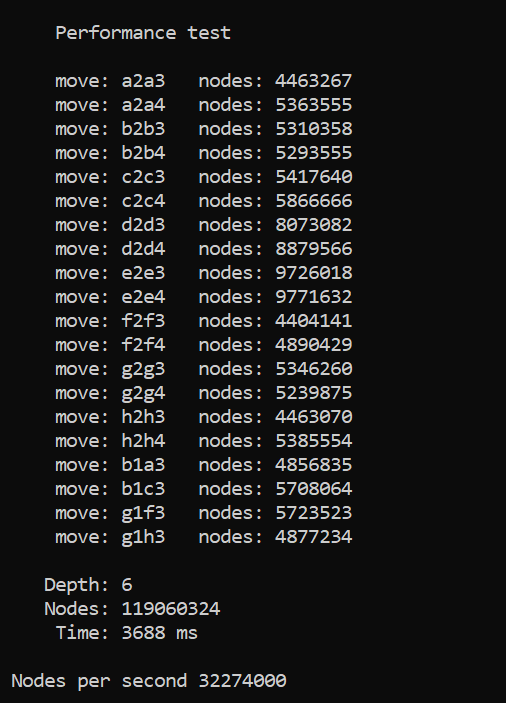
\includegraphics{perftscore.png}
    \caption{Output tipico di una funzione di perft,il numero di nodi viene diviso per sottoalbero di appartenenza per facilitare il debugging, il numero di nodi al secondo (32.27M) può essere utilizzato come metrica prestazionale.}
    \label{perftscore}
\end{figure}


\section{Ricerca} \label{ricerca}
Una volta generate tutte le possibili mosse nella fase di move generation si entra nella fase di ricerca,che consiste nel eseguire diversi sottoinsiemi delle possibili mosse e valutare
lo stato della scacchiera per trovare le mosse che forniscono il risultato finale migliore. Possiamo dire in maniera più tecnica che , essendo il gioco degli scacchi un gioco
a 2 giocatori,a informazione perfetta e a somma zero, la ricerca implica l'attraversamento e l'ottimizzazione di un albero mini-max contenente le possibili posizioni di gioco.
Negli scacchi computazionali esistono due approcci alla progettazione di un algoritmo di ricerca,si può effettuare una ricerca a tappeto limitando la profondità
della stessa per far si che i calcoli finiscano in tempi accettabili ,col rischio di sottovalutare implicazioni future di determinate mosse,o focalizzarsi su particolari mosse e quindi
rami dell'albero di ricerca nel tentativo di dare maggiore spazio alle mosse migliori (sulla base dell'euristica scelta per determinare come sia fatta una mossa "migliore"), rischiando
quindi di eliminare a priori mosse con dei risvolti successivi molto promettenti,l'approccio adottato da quasi tutti i motori scacchistici moderni è il primo.

\subsubsection{Algoritmi di ricerca}
Data l'impossibilità di esplorare l'intero spazio dell'albero di ricerca che codifica il gioco degli scacchi, è necessario fare affidamento ad algoritmi in
grado di ridurre il numero di nodi dell'albero, l'approccio più utilizzato è quello di una ricerca minimax con potatura alfa-beta ad approfondimento iterativo.


\subsubsection{Minimax e negamax}
L'algoritmo minimax\cite{itwiki:125837390} è un algoritmo ricorsivo per la ricerca della mossa migliore in una determinata situazione, si basa su una funzione di valutazione posizionale che assegna ad una posizione (rappresentante un possibile stato del gioco) un punteggio,
che indica quanto è desiderabile per il giocatore raggiungere quella posizione.
L'obbiettivo finale è la minimizzazione (mini) del massimo guadagno del giocatore avversario (max),
l'algoritmo minimax quindi  assegna un valore ad ogni mossa , proporzionale a quanto essa diminuisce il valore della posizione per l'altro giocatore,
l'effettivo valore che viene assegnato dipende dalla funzione di valutazione adottata,\emph{questo argomento verrà trattato successivamente nella parte dedicata alla valutazione}.
L'algoritmo minimax è in grado di formulare una strategia perfetta per giochi abbastanza semplici da poter permettere 
la valutazione dell'intero albero di ricerca, per giochi complessi come gli scacchi però questo non è possibile o lo è 
solo nelle fasi finali e ,in generale, si può solo calcolare una stima della probabilità che una data mossa porti alla vittoria di uno dei giocatori.
Il calcolo di questa stima può essere migliorato se è possibile fornire una funzione di valutazione euristica che
valuti le posizioni non terminali del gioco senza dover conoscere tutte le mosse successive: in questo caso si possono
considerare solo un certo numero di mosse future. Questo numero è detto "profondità" dell'algoritmo ed è misurato
in mosse. il numero di nodi da valutare cresce esponenzialmente con la profondità di ricerca La complessità computazionale dell'algoritmo minimax è quindi 
NP completa, il che lo rende poco pratico per ottenere una soluzione definitiva di giochi meno che banali,tuttavia, le prestazioni del minimax possono essere migliorate drasticamente,
mantenendo la correttezza dei risultati, adottando la \textbf{potatura alfa-beta}.
\\Negamax è una variante dell'algoritmo minimax che si basa sulla nozione che $max(a,b)= -min(-a,-b)$ per semplificare l'implementazione dell'algoritmo minimax,
in pratica, il valore di una posizione per il giocatore A è l'opposto di segno di quello del giocatore B, quindi il giocatore che muove deve puntare a massimizzare il valore negato della posizione
dopo la sua mossa, questo tipo di ragionamento è applicabile sia per il giocatore minimizzante che per quello massimizzante, questo modo di operare permette di non dover implementare due funzioni diverse per i due agenti 
e di ridurre il tutto ad un solo algoritmo.



\subsubsection{Potatura alfa-beta}
La potatura alfa-beta è un algoritmo di ricerca utilizzato per ridurre il numero di nodi valutati dall'algoritmo 
minimax,consiste nello smettere di esaminare una mossa, e con essa tutte le mosse derivanti da essa a profondità maggiori
(i rami del nodo mossa,che vengono quindi "potati"), quando si rivela peggiore di una mossa già esaminata precedentemente,
abbiamo quindi la rimozione di solo mosse ininfluenti per quanto riguarda l'albero minimax e quindi la mossa
restituita dopo l'implementazione della potatura alfa-beta sarà equivalente a quella restituita da un algoritmo
minimax senza potatura.

\subsubsection{Approfondimento iterativo}
In ogni variante degli scacchi troviamo un elemento di limitazione temporale, il cosiddetto controllo del tempo\footnote{il controllo del tempo è quanto tempo è assegnato al giocatore
per poter effettuare le sue mosse,può essere statico, quando tutto il tempo viene assegnato fin dall'inizio ad ogni giocatore, che può gestirlo come più preferisce,o dinamico, 
quando il tempo può aumentare dopo determinati punti chiave,come ad esempio l'aver eseguito una o più mosse.},
questo limite temporale implica chiaramente la necessità di dover ad un certo punto il dover cessare di pensare alla 
possibile mossa migliore ed eseguire la migliore che si è trovata fino a quel momento.
A livello implementativo risolvere questo problema si tramuta nella necessità di implementare una componente di approfondimento
iterativo all'interno del nostro algoritmo di ricerca.
L'approfondimento iterativo consiste nell'effettuare la ricerca all'interno di un albero fino ad una data profondità n,
terminata la ricerca a profondità n si effettua una ricerca a profondità n+1, n+2 e via via si aumenta la profondità tempo permettendo,
questo permette di avere un risultato da restituire indipendentemente dal tempo, a patto che sia sufficiente a completare una 
ricerca ad almeno profondità 1 (si tratta generalmente di nanosecondi e quindi di tempo che si ha sempre a disposizione), il lato negativo
è quello di dover ripetere la ricerca su livelli già precedentemente esplorati,tuttavia esistono tecniche in grado di alleviare questo scotto prestazionale,
possiamo utilizzare informazioni apprese durante le precedenti visite per guidare quelle successive e ridurre al minimo la parte da dover ri-esplorare.
Le principali euristiche ottenute dalle visite precedenti prendono il nome di \textbf{euristica killer} e \textbf{euristica storica}.
\begin{itemize}
  \item  \textbf{euristica killer}: una mossa killer è una mossa che non cattura nessun pezzo e che causa un taglio beta\footnote{quando la ricerca trova 
  una posizione con una valutazione  superiore a beta, significa che in fasi precedenti della ricerca è stato trovato un percorso utilizzabile 
   dall'avversario che risulta in un punteggio finale peggiore per l'avversario,questo significa che,supponendo un gioco
   perfetto da parte di entrambi i giocatori, il giocatore avversario non finirà mai nel sotto-albero contente tale mossa e che quindi si 
   può procedere all potatura},si salvano generalmente un paio di mosse killer per ogni profondità dell'albero di ricerca e nelle successive iterazioni
   verranno eseguite con una priorità maggiore rispetto alle altre mosse per accelerare la ricerca. 
  \item \textbf{euristica storica}: l'euristica storica è un euristica che si basa sul numero di miglioramenti di alfa che quella mossa ha causato
   durante la ricerca,si tratta nuovamente di un tipo di mossa che non cattura nessun pezzo ed inoltre non deve produrre un taglio beta
  (verrebbe altrimenti classificata come mossa killer), è generalmente conservata come coppia pezzo/casella in cui il pezzo si muove 
  ed anch'essa  nelle successive iterazioni verrà eseguite con una priorità maggiore rispetto alle altre mosse per accelerare la ricerca. 
\end{itemize} 
euristiche come quella storica o quella killer fanno a loro volta parte di un problema più grande e fondamentale per gli scacchi computazionali 
e la potatura alfa-beta in generale,si parla del problema dell'ordinamento delle mosse.

\subsubsection{Ordinamento delle mosse}
Come abbiamo precedentemente visto con l'euristica storica e l'euristica killer,provare prima una mossa "forte" ossia una mossa in grado di 
poter migliorare alpha o causare un taglio beta ci permette di aumentare enormemente l'efficacia della potatura alfa-beta e diminuire in maniera 
sensibile lo spazio di ricerca, l'ordinamento delle mosse tenta di massimizzare il guadagno possibile dall'utilizzo di mosse "forti" utilizzando 
diverse metriche per selezionare mosse da provare prima delle altre.Un esempio di gerarchia tipica di ordinamento delle mosse è:
\begin{itemize}
\item la mossa migliore in una posizione individuata in una ricerca precedente a profondità minore.
\item mosse dalla tabella  di trasposizione.
\item catture e promozioni.
\item mosse killer
\item mosse che non catturano pezzi ordinate secondo l'euristica storica.
\end{itemize} 
È inoltre possibile utilizzare euristiche per ordinare tra di loro mosse appartenenti allo stesso livello,non è raro infatti optare di ordinare le catture da più promettenti a meno promettenti,
l'euristica principale per stabilire quanto una cattura è definibile promettente prende il nome di \textbf{mvv-lva} o in forma estesa \textbf{most valuable victim / least valuable attacker} ,l'obbiettivo è quello di identificare 
il pezzo di minore importanza che può attaccare il pezzo di maggiore importanza,ai due estremi troviamo un pedone in grado di catturare una regina ed una regina che viene scomodata per catturare un semplice pedone,
l'ordinamento preferisce intrinsecamente il tipo del pezzo attaccante, quindi tutte le mosse di cattura effettuabili da un pedone verranno considerate prima di quelle di un cavallo che a loro volta verranno considerate
prima di quelle di un alfiere e cosi via fino ad arrivare ad una regina. 


\subsubsection{Effetto orizzonte e ricerca di quiescenza}
L'effetto orizzonte è un problema che affligge tutti gli algoritmi di ricerca con profondità limitata,l'orizzonte è la divisione 
tra le mosse considerate dal nostro algoritmo di ricerca e quelle  che si trovano ad una profondità maggiore rispetto a quella raggiunta dal nostro algoritmo 
ed il problema nasce dall'impossibilità di poter analizzare le conseguenze delle mosse che si ritengono forti agli ultimi livelli di profondità, in quanto dovendo fermarci con la ricerca,
non possiamo indagare eventuali risposte avversarie.\\
Immaginiamo di trovarci in una posizione di gioco immaginaria chiamata k , e di cercare tutte le possibili posizioni derivanti da k con una profondità pari a 5,
chiameremo k+5 la migliore delle posizioni raggiunte da queste ricerca sulla base della funzione di valutazione,è possibile che
l'avversario abbia una mossa con la quale può ribaltare istantaneamente la bontà della posizione k+5, trasformandola quindi in una posizione
"k+6" molto più sfavorevole.\\
Un esempio classico di questo problema in ambiente scacchistico è quello di una ricattura: immaginiamo 
di effettuare una ricerca più superficiale possibile, a profondità 1, in questo stato qualsiasi cattura terminerà con un miglioramento di punteggio 
per la posizione del giocatore che muove (in quanto ha appena catturato un pezzo avversario),supponiamo quindi ad esempio di aver catturato un pedone con una regina,
l'effetto orizzonte non ci permette di vedere a profondità 2 o oltre le conseguenze di questa azione,qualora quel pedone fosse stato 
protetto da qualsiasi altro pezzo, il nostro avversario potrà in risposta alla cattura del pedone catturare la regina attaccante,
si passerebbe quindi dall'aver guadagnato un pedone all'aver perso una regina, un cambio di valutazione estremo e repentino,questo problema che è estremamente esacerbato a profondità 1 è presente a tutti i livelli di ricerca e rende un motore che non applica misure per contenerlo 
non in grado di giocare ad un livello soddisfacente. 
\\Un modo per tentare di ovviare a questa soluzione prende il nome di \textbf{ricerca di quiescenza}, una ricerca che entra in gioco quando abbiamo raggiunto la massima 
profondità possibile dalla ricerca alfa-beta e serve a cercare una posizione "calma", senza forti variazioni di valutazione nei turni successivi,il modo più facile di implementarla consiste nel proseguire con la ricerca
alfa-beta a partire dalla massima profondità raggiunta dalla ricerca alfa-beta ma considerando solo le mosse di cattura , la generazione delle sole catture implica che il fattore di diramazione dell'albero è fortemente ridotto e quindi la 
ricerca non è particolarmente impegnativa (rispetto alla ricerca alfa-beta madre), al termine di questa ricerca viene restituita una nuova valutazione, che sarà poi considerata la valutazione finale di ogni posizione.


 


\subsubsection{Ricerca a variazione principale}
La Ricerca a variazione principale, chiamata anche \textbf{PVS (principal variation search)}, conosciuta anche come NegaScout, è un algoritmo di tipo negamax che può essere più veloce della potatura alfa-beta 
in quanto non considera  mai nessun nodo che può essere potato dalla potatura alfa-beta, PVS si base sull'assunzione che le mosse siano state ordinate in maniera corretta e produce un numero maggiore di tagli
dando per scontato che il primo nodo esplorato sia il migliore di quelli possibili,una ricerca di questo tipo è molto più veloce di una ricerca che si preoccupa che una delle possibili mosse restanti possa essere 
buona, se però viene trovato un nodo migliore allora è necessario ri-effettuare una ricerca normale alfa-beta su quel nodo, in pratica quindi, per ogni nodo ordinato in maniera sbagliata si deve ripetere la ricerca, e 
con abbastanza ricerche ripetute diventa più lento di alfa-beta pur esplorando lo stesso numero di nodi , è per questo che la ricerca ha bisogno di un ordinamento il più accurato possibile.
In termini pratici una ricerca PVS si realizza utilizzando una ricerca alfa-beta ma con una finestra nulla al posto dei normali parametri alfa e beta,all'interno di un contesto negamax una finestra nulla è un 
intervallo alfa-beta dove beta vale alpha-1.



\subsubsection{Transposition Table e Hashing Zobrist}
Non è raro per un motore scacchistico incontrare multiple volte, durante la fase di ricerca, la stessa posizione, sia per pezzi con mosse "reversibili" in grado quindi di far tornare la ricercare al nodo padre,
causando un potenziale ciclo, sia perchè è possibile giungere ad una posizione finale identica percorrendo multiple strade, immaginiamo ad esempio le mosse a2a4-a7a5 e d2d4-d7d5, non importa l'ordine di esecuzione,
la posizione finale vedrà in ogni caso un pedone bianco su a4 e su d4 ed un pedone nero su a5 e su d5.
\\ Una \textbf{tabella di trasposizione} è una tabella hash che conserva i risultati di ricerche precedentemente effettuate
su una data posizione, ogni volta che si raggiunge una nuova (per l'iterazione locale del processo di ricerca) posizione, si cerca all'interno di questa tavola dei risultati precedenti associati a tale posizione, in caso di riscontro positivo
vengono prelevati i dati risalenti all'ultima ricerca effettuata, spesso composti da posizione, profondità e punteggio finale della ricerca.
\\Per individuare una posizione all'interno della tabella si utilizza una chiave hash in grado di codificare univocamente una posizione su una scacchiera, per la generazione di queste chiavi una tecnica molto diffusa prende il nome di hashing zobrist, 
nell'hashing zobrist si assegna una chiave casuale di 64 bit ad ogni combinazione pezzo-posizione, ad ogni possibile insieme di permessi di arrocco, ad ogni possibile casella di en passant ed ai due lati di gioco possibili (bianco e nero),
si parte poi da una chiave vuota e man mano vengono inseriti tramite XOR bit a bit, le chiavi dei pezzi presenti sulla scacchiera corrispondenti alle posizioni in cui si trovano, degli attuali permessi di arrocco
del lato giocante e dell'eventuale casella di enpassant,data però data l'impossibilità di contenere tutte le possibili chiavi all'interno di una tabella hash,si utilizzano metodi per ridurre l'universo delle chiavi,
il più banale e comune rappresentato dall'effettuare il modulo della chiave zobrist originale col numero di istanze massime nella tabella,per via di questa limitazione è possibile che avvengano delle collisioni,
in quanto due chiavi zobrist diverse possono generare la stessa chiave hash post modulo,per ovviare a questo problema è necessario controllare che la chiave zobrist corrisponda a quella salvata nella tabella di 
trasposizione ad ogni accesso, ed in caso contrario effettuare la sovrascrittura dell'istanza precedentemente inserita.



\section{Valutazione}
Nelle sezione di ricerca abbiamo incontrato per la prima volta la necessità di valutare una posizione tramite una funzione di valutazione,in modo da poter guidare la ricerca verso soluzioni dal punteggio 
migliore rispetto ad altre,per parlare di ricerca però abbiamo visto la funzione di valutazione come una scatola nera,ci bastava semplicemente sapere che esisteva una funzione che data una posizione qualsiasi 
era in grado di restituire un numero che ne rappresentasse la bontà, in realtà la funzione di valutazione è il pezzo più complesso e delicato di un motore,in grado da sola di distinguere un pessimo motore
da uno dei migliori al mondo, per questo è necessario, quando si lavora alla formulazione di una funzione del genere,lavorare in maniera graduale e testare ampiamente ogni modifica che si apporta.

\subsubsection {hand-crafted evaluation}
Si definisce hand-crafted evaluation, abbreviata in HCE e traducibile con "valutazione fatta a mano",una funzione di valutazione che considera diversi aspetti della posizione ed assegna ad ognuno di essi un peso 
arbitrario deciso dallo sviluppatore (da qui il termine hand-crafted), si tratta della metodologia classica per la scrittura di una funzione di valutazione ed ancora oggi si dimostra estremamente popolare in  
motori di tutti i livelli, anche se sta man mano venendo soppiantata dall'utilizzo di reti neurali, come constatabile nella crème de la crème dei motori scacchistici (Stockfish, Lc0,Dragon), l'approccio più comune
nella realizzazione di una funzione di valutazione HCE consiste nell'effettuare una combinazione lineare di diverse euristiche indipendenti, ognuna riguardante un aspetto più o meno fondamentale di una posizione.
\\La prima è più banale euristica che possiamo considerare è quella del valore dei pezzi, si assegna ad ogni pezzo un valore numerico espresso in centesimi di pedone che ne individua l'importanza \footnote{Si riportano ad esempio i valori individuati
da Alan Turing nel 1953: Pedone:100, Cavallo:300, Alfiere:350, Torre:500, Regina:1000},il valore di una posizione per un dato giocatore sarà espresso dalla somma dei valori dei suoi pezzi meno la somma dei valori dei pezzi avversari.
Questo approccio da solo è utile per evitare che  pezzi fondamentali come la regina vengano lasciati in balia delle mosse avversarie ma allo stesso tempo è insufficiente nel guidare le mosse del motore in fase di attacco,
fermandosi qui ci si ritroverebbe con un motore che scappa costantemente dal confronto ed accetta di tanto in tanto degli scambi di materiale senza puntare ad una conclusione e senza nessun approccio tattico.
Un'altra euristica molto banale e di facile implementazione si basa sull'associare ad ogni coppia pezzo-casella un valore, che verrà poi sommato al valore intrinseco del pezzo stesso,questo valore può essere positivo
per incentivare lo spostamento di un pezzo in una determinata casella o negativo per ottenere l'effetto opposto,la positività e la negatività di un valore associato ad una casella sono un tentativo di inserire 
nozioni scacchistiche di base all'interno dell'algoritmo per meglio guidarne le scelte,ad esempio, è comunemente risaputo che un cavallo ha molto più valore al centro, dove può sfruttare tutta la sua mobilità 
con un massimo possibile di 8 mosse e non ad un angolo della scacchiera, dove almeno 4 di quelle mosse  (tutte quelle che vanno verso il bordo sul quale il cavallo si trova) vengono perse.

\begin{figure}
    \centering
    \includegraphics{immagine.png}
    \caption{esempio di valori associati alle caselle della scacchiera per un cavallo conservati in un array del linguaggio C}
\end{figure}

L'ultima euristica che andremo a considerare,in quanto è impossibile elencarle tutte ed è anche controproducente in quanto la natura scacchistica delle stesse richiede conoscenze che non possono essere facilmente riassunte
, riguarda la posizione dei pedoni,un pedone può godere di tre caratteristiche in grado di cambiarne il valore, un pedone può essere infatti  un pedone passato, doppiato o isolato.\\
Un pedone passato è un pedone che non può essere contrastato nella marcia in avanti da un pedone avversario sia sulla stessa colonna, sia a destra o a sinistra di essa,questo tipo di pedone quindi può facilmente 
minacciare un'avanzata verso la fila posteriore nemica con lo scopo di promuovere,un pedone passato è un pezzo particolarmente utile nel fine gioco ed in quanto tale gli viene conferito un punteggio migliore
rispetto a quello di un normale pedone .\\ 
Un pedone doppiato è un pedone che, a seguito di una presa, passa nella fila vicina dove si trova un altro pedone dello stesso colore,si tratta generalmente di una debolezza strutturale di una posizione 
ed in quanto tale va evitata se non porta a vantaggi sostanziali,spesso quindi si assegna ad ogni pedone doppiato un malus di punteggio.\\
Un pedone isolato è un pedone che nel corso della partita rimane senza pedoni sulle due colonne adiacenti, si tratta quindi di un pedone che non può essere difeso dai pedoni adiacenti e quindi di un pezzo
facilmente attaccabile per l'avversario, per questo è prassi assegnare ad ogni pedone isolato un malus di punteggio.
In termini pratici una realizzazione tipica di questa euristica si basa sulla generazione di bitmask statiche che in combinazione con la bitboard dei pedoni saranno in grado di identificare queste tipologie di pedoni.



\section {Libro delle aperture e Tablebase}
Le mosse iniziali di una partita di scacchi, chiamate nel loro insieme "apertura" posseggono un particolare binomio di caratteristiche, si tratta di mosse che avvengono in posizioni estremamente aperte,con tutti o quasi i pezzi
in gioco e quindi con moltissime possibilità da calcolare, allo stesso tempo si tratta di alcune tra le mosse più studiate in ambito di teoria scacchistica nel corso dei secoli, è prassi quindi quella di evitare che
il calcolatore elabori da se le prime mosse e far si che si appoggi su un database di mosse di apertura chiamato appunto libro delle aperture, che contiene solitamente aperture che vanno dalle 4 alle 10-11 mosse.
Seguendo ancora il paradigma di risparmiare al motore parti di calcolo basandosi su mosse precompilate,ma con un caso d'uso diametralmente opposto, ossia quando la posizione di gioco è abbastanza semplice
da poter enumerare ogni possibile mossa e calcolare a priori il miglior risultato possibile per un determinato giocatore, nascono le tablebase, database esaustivi di mosse pre-calcolate delle fasi finale di una 
partita, ad oggi sono disponibili tablebase complete fino a 7 pezzi presenti sulla scacchiera, questo significa che, per un numero di pezzi compreso tra 3 e 7, non importa quali o in disposti in quale modo,
è possibile conoscere da subito l'esito della partita (presupponendo un gioco perfetto).
